\documentclass[
	12pt,
	a4paper,
	onepage,
	brazil
]{article}

\usepackage[brazil]{babel}
\usepackage[utf8]{inputenc}
\usepackage[T1]{fontenc}
\usepackage{lmodern}
\usepackage{hyperref}
\usepackage{amsmath}
\usepackage{amsthm}
\usepackage{amsfonts}
\usepackage{indentfirst}
\usepackage[most]{tcolorbox}
\usepackage{inconsolata}
\usepackage{caption}
\usepackage{floatrow}
\usepackage[lined,algonl,ruled]{algorithm2e}
\usepackage{float}
\usepackage{graphicx,url}
\usepackage{times,epsfig}
\usepackage[
	backend=bibtex8,
	style=numeric
]{biblatex}
\addbibresource{tp2.bib}
\usepackage{xcolor}
\hypersetup{
	colorlinks,
	linkcolor={red!50!black},
	urlcolor={red!80!black}
}

\usepackage[
	lmargin = 25mm,
	rmargin = 25mm,
	tmargin = 25mm,
	bmargin = 25mm
]{geometry}

\usepackage{mathtools}
\DeclarePairedDelimiter\ceil{\lceil}{\rceil}

\sloppy

\author{Pedro Otávio Machado Ribeiro}
\title{Trabalho Prático 3\\Legado da Copa
	\\Algoritmos e Estruturas de Dados III - 2017/01}
\date{10/07/2017}

\begin{document}

	\maketitle
	
	\section{Introdução}
	
	Neste trabalho temos como contexto uma rua muito movimentada chamada Rua Pai no Bar, que, sugestivamente, possui muitos bares. Os donos dos bares desta rua moram no lado da rua oposto ao bar para que possam verificar facilmente qualquer movimentação suspeita. Para não falhar com a tradição, os donos dos bares querem pendurar bandeirolas para alegrar a vizinhança, já que a Copa na Rússia está chegando. Como os donos dos bares foram afetados pela crise, cada um fornecerá apenas uma bandeirola que pode ser pendurada de sua casa até seu bar, porém uma bandeirola não pode se cruzar com a outra. Logo, dado uma lista de tamanho $n$ de pares de números que representam o bar e a casa do dono, o objetivo deste trabalho é encontrar o maior número de bandeirolas que pode-se pendurar, respeitando as condições acima descritas. A númeração das ruas ocorre da forma usual: um lado com números pares, e o outro com números ímpares. Como este trabalho trata-se de paradigmas, a meta é solucionar este problema utilizando três técnicas diferentes: Força Bruta, Guloso e Programação Dinâmica.
	
	\section{Metodologia}
	
	Como foi pedido, este problema foi solucionado por meio de 3 métodos diferentes: Força Bruta, algoritmo Guloso - que neste caso não se aplica, mas foi feita uma heurística para aproximar a resposta - e Programação Dinâmica.
	
	Para representar um par de bar e seu dono, foi feita uma estrutura de dois números, em que o primeiro é o maior e o segundo, o menor. Logo, uma rua é representada por um vetor desta estrutura, e, antes de executar qualquer um dos métodos, este vetor é ordenado pelo primeiro elemento de cada estrutura. Desta forma, as bandeirolas ficam ordenadas pela posição em que ela termina.
	
	Para detectar os cruzamentos, independentemente se o bar fica no lado ímpar ou par, sem perda de generalidade, basta comparar as coordenadas pares das bandeirolas e as ímpares, pois, apesar de tudo, bar e dono do bar são apenas nomes para os extremos das bandeirolas. A verificação é dada da seguinte forma:
	
	Seja $A = (p_a, i_a)$ e $B = (p_b, i_b)$ as bandeirolas representadas por um número par $p$ e ímpar $i$ que dizem a posição das extremidades em cada lado da rua. $A$ e $B$ não se cruzam se, e somente se, $(p_a > p_b \land i_a > i_b) \lor (p_a < p_b \land i_a < i_b)$. Em outras palavras, uma bandeirola está a frente, ou atrás de outra.
	
	Dado isso, segue abaixo a descrição da solução por meio de cada método.
	
	\subsection{Força Bruta}
	
	Para solucionar o problema com um algoritmo de força bruta, basta incluir ou não uma bandeirola. Dado que inicialmente o vetor de bandeirolas foi ordenado como descrito, se uma bandeirola $b_i$ não se cruza com uma bandeirola $b_{i-1}$, então a bandeirola $b_i$ não se cruzará com nenhuma das bandeirolas $b_k$, onde $k \in [0, i-1[$. Dessa forma, uma bandeirola é adicionada à uma combinação se ela satisfaz essa condição, proporcionando assim, uma poda que impede que uma combinação com cruzamento seja formada.
	
	Note que, no pior caso, todas as combinações possíveis serão verificadas, percorrendo assim, todo o espaço solução. O número de combinações possíveis pode ser representado análogamente pelo o que conhecemos como conjunto pontência, em que seu tamanho é $2^n$, onde $n$ é o número de bandeirolas, neste caso.
	
	\subsection{Guloso}
	
	Dado que este problema não possui solução gulosa ótima, uma heurística que aproxima a solução foi desenvolvida.
	
	A heurística feita para aproximar a solução é simples. Assuma que a primeira bandeirola $b_k, k = 0$ faz parte da combinação solução de bandeirolas. Em seguida, para cada bandeirola $b_i, i \in [1, n-1]$, $b_i$ pertence a combinação solução se, e somente se ela não cruza com a bandeirola $b_k$ onde $k$ é o índice do último elemento adicionado na combinação solução, caracterizando, assim, uma escolha gulosa. O mesmo procedimento é realizado de trás pra frente, assumindo-se inicialmente que a última bandeirola faz parte da solução. Ao final, a combinação que tiver o maior tamanho é escolhida e definida como resposta.
	
	\subsection{Programação Dinâmica}
	
	Dado que temos o vetor de bandeirolas ordenado pelo término, para saber quantas bandeirolas é possível pendurar até a bandeirola $i$, devemos encontrar a última bandeirola $j \in [0, i-1]$ tal que $i$ não cruza com $j$ e a solução para $j$ é a maior possível. Assim como explicado na força bruta, se a bandeirola $i$ não se cruza com a $j$, então $i$ não se cruza com nenhum que venha antes de $j$. Logo, a solução da programação dinâmica se dá pela seguinte equação de recorrência:
	
	\begin{equation}
		dp(i) = \begin{cases} 1, & \mbox{if } i = 0 \\ max(dp(j)) + 1, \forall j \in [0, i-1], & \mbox{if } i \ne 0\end{cases}
	\end{equation}
	
	\section{Complexidade}
	
	\subsection{Temporal}
	
	\subsubsection{Força Bruta}
	
	O algoritmo de força bruta, na forma como foi feito, tem como pior caso a combinação em que todas as bandeirolas são inclusas, representado pelo último galho da árvore de recursão. Dessa forma, nenhuma poda acontecerá, e todas as $2^n$ combinações possíveis serão testadas, percorrendo assim todo o espaço de solução. Logo, a complexidade temporal do algoritmo de força bruta será $O(2^n)$.

	\subsubsection{Guloso}
	
	Dado que para obter a solução aproximada o vetor de bandeirolas é percorrido necessariamente duas vezes, assintóticamente o custo temporal da solução é $O(n)$.
	
	\subsubsection{Programação Dinâmica}
	
	Para cada bandeirola $i$ o algoritmo faz uma busca linear para encontrar a última bandeirola $j$ que satisfaz as condições mostradas. No pior caso, a busca terá complexidade $O(n)$. Como a busca é realizada $n$ vezes, a complexidade assintótica do algoritmo de programação dinâmica será dado por $O(n^2)$.
	
	\subsection{Espacial}
	
	Todos os algoritmos desenvolvidos no máximo 2 vetores de tamanho máximo $n$. Logo, assintóticamente, o uso de memória é dado por $O(n)$.
	
	\section{Experimentos}
	
	Os testes foram realizados em meu computador pessoal, um notebook que não é mais um notebook, com as seguintes configurações:
	
	\begin{itemize}
		\item Sistema Operacional: Arch Linux
		\item Processador: Intel(R) Core(TM) i5-2430M CPU @ 4 $\times \ $2.40GHz
		\item Memória RAM: 6GB
	\end{itemize}
	
	Cada teste foi realizado 10 vezes e os valores apresentados são referentes a média destes.
	
	Os casos de teste utilizados foram gerados por mim, utilizando um algoritmo que fornece uma entrada dado um tamanho $n$.
	
	O tamanho dos casos de teste variam de 22 a 31 para o algoritmo de força bruta, de forma que o algoritmo sempre caia no pior caso, favorecendo assim uma melhor visualização dos dados. Segue abaixo o gráfico de tempo de execução:
	
	\begin{figure}[H]
		\centering
		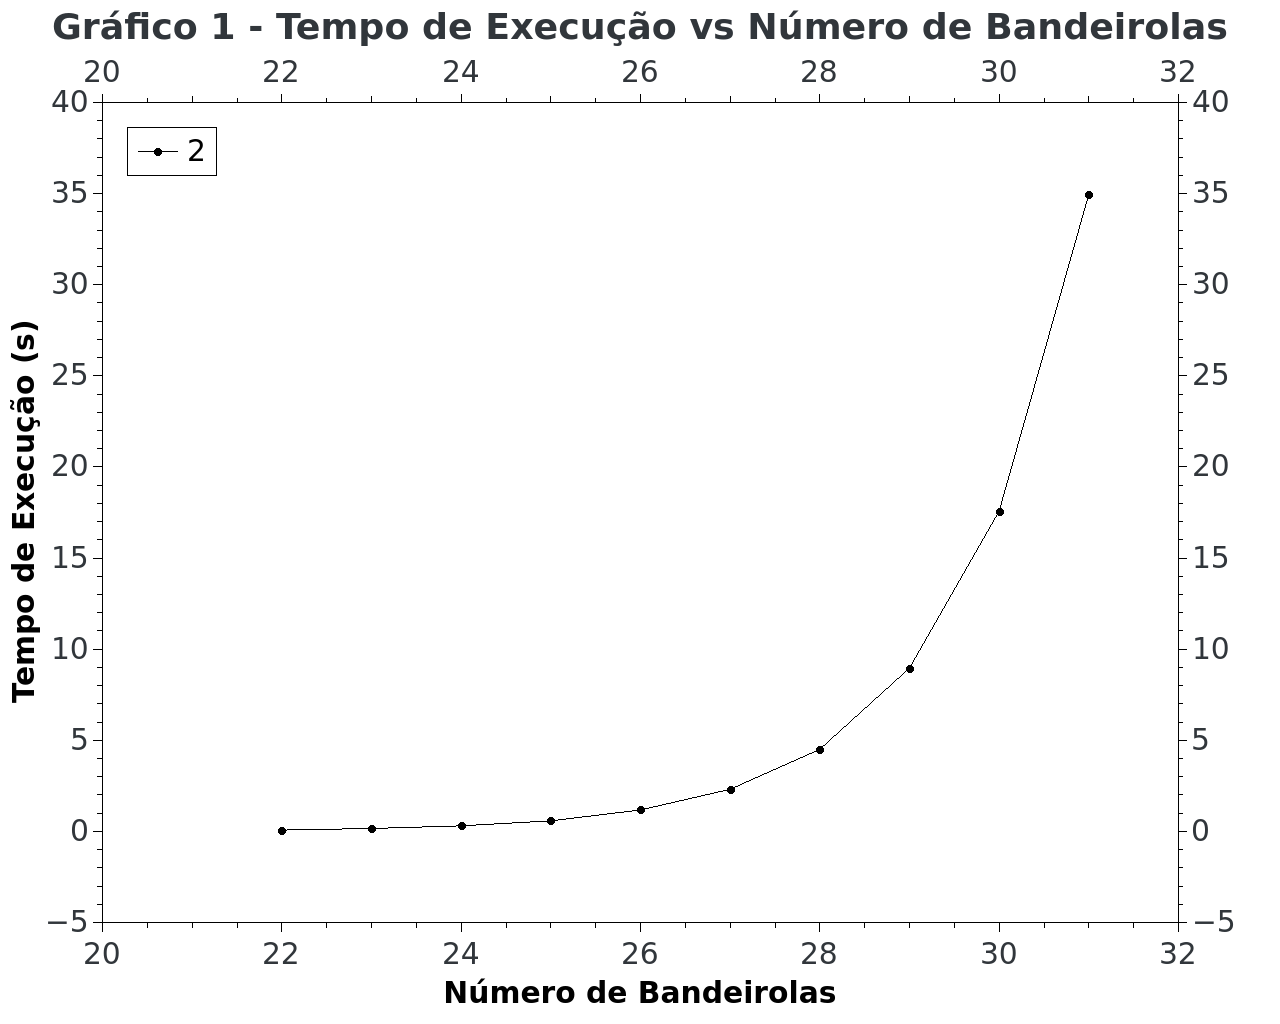
\includegraphics[scale=2]{brute_force_graph.png}
		\caption{Tempo de Execução em função do Número de Bandeirolas para o força bruta}
	\end{figure}

	Para o algoritmo guloso, o tamanho dos casos de testes variam de 10000 a 14500, aumentando 500 a cada nova instância. Segue abaixo o gráfico de tempo de execução:
	
	\begin{figure}[H]
		\centering
		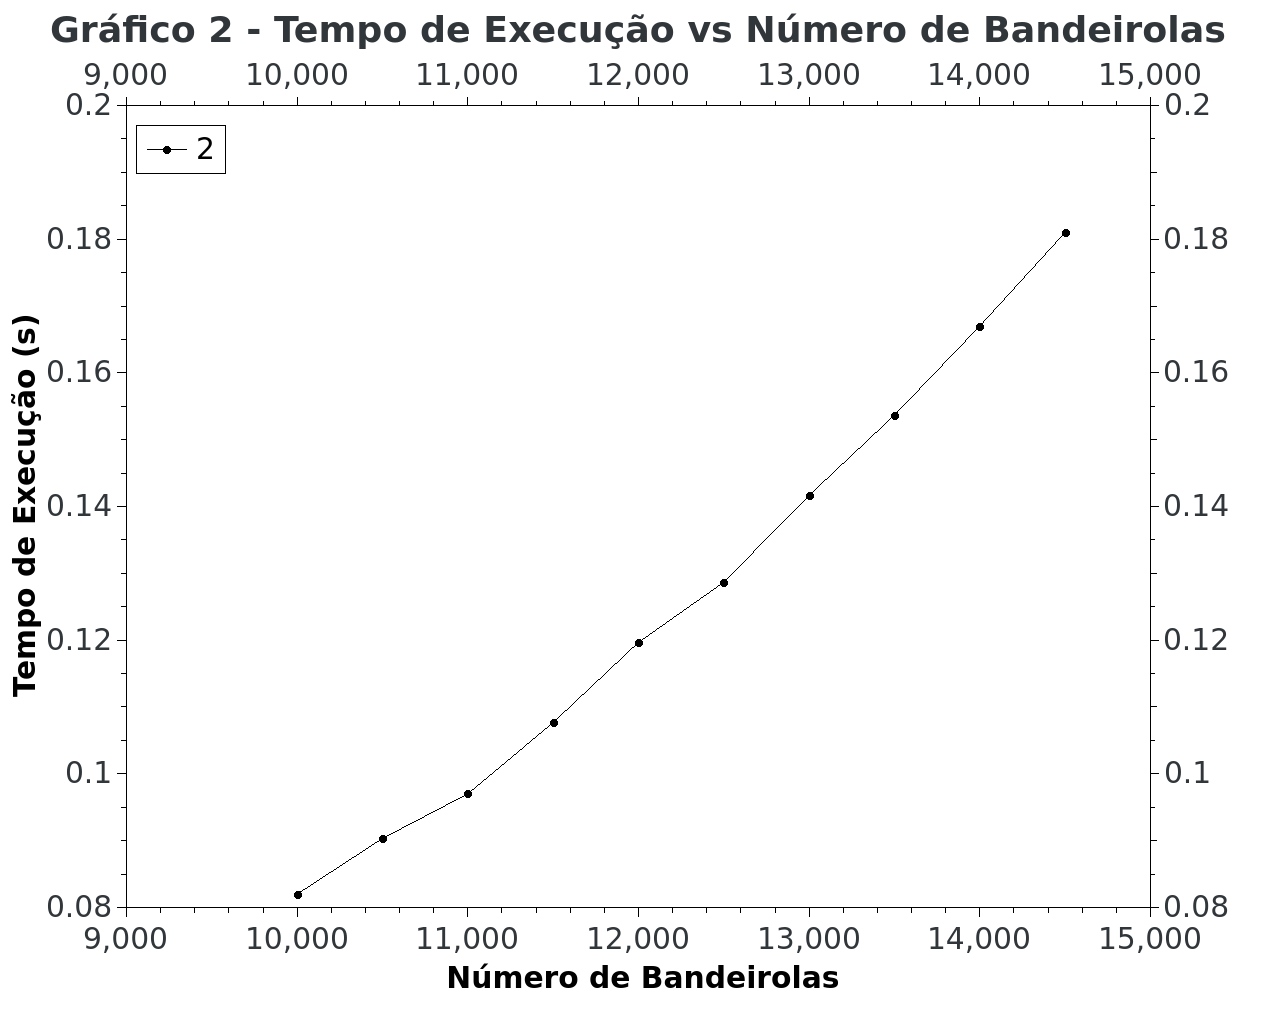
\includegraphics[scale=2]{greedy_graph.png}
		\caption{Tempo de Execução em função do Número de Bandeirolas para o guloso}
	\end{figure}

	Analogamente, os testes utilizados para a programação dinâmica possuem as mesmas características, porém o tamanho dos casos de teste varia de 10000 a 100000, aumentando 10000 a cada nova instância. Segue abaixo o gráfico de tempo de execução:
	
	\begin{figure}[H]
		\centering
		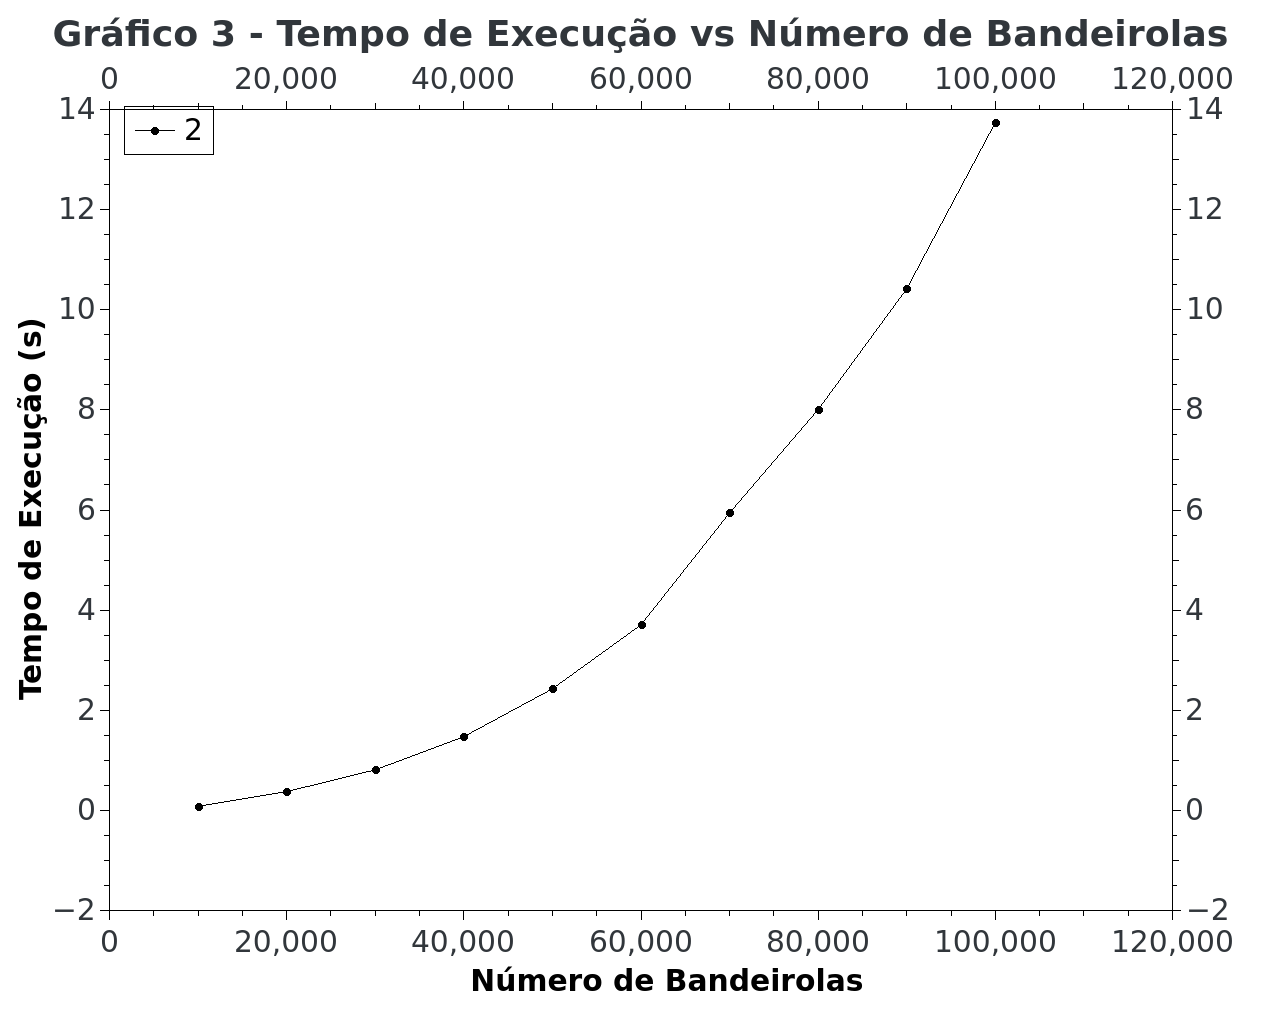
\includegraphics[scale=2]{dp_graph.png}
		\caption{Tempo de Execução em função do Número de Bandeirolas para a PD}
	\end{figure}
	
	\section{Análise de Resultado}
	
	Nota-se que para o algoritmo de força bruta o gráfico demonstra um comportamento exponencial, bem como esperado dado que sua complexidade temporal é $O(2^n)$.
	
	Para o algoritmo guloso, os testes mostram um comportamento linear conforme o tamanho da entrada aumenta, corroborando assim seu comportamento assintótico definido por $O(n)$.
	
	Finalmente, para a programação dinâmica, podemos observar o corportamento polinomial de grau 2 mostrado no terceiro gráfico, condizendo, assim, com a complexidade do algoritmo, que é $O(n^2)$.
	
	\section{Conclusão}
	
	Nota-se, por meio deste trabalho, que um mesmo problema pode ser solucionado utilizando paradigmas diferentes. Para este problema de pendurar bandeirolas, foram apresentados as soluções por meio de força bruta, guloso e programação dinâmica. 
	
	O algoritmo força bruta fornece o resultado ótimo, porém este torna-se inviável de ser utilizado quando o número de bandeirolas é grande. 
	
	Por outro lado, o algoritmo guloso, que neste caso é uma heurística que tenta se aproximar da resposta ótima, mostra-se mais eficiente, no entanto ainda pode ser melhorada, dado que há outras características que podemos tirar vantagem, como a distância entre bandeirolas. 
	
	Finalmente, temos a programação dinâmica, que apesar de ser polinomialmente maior que o guloso, compensa apresentando sempre a resposta ótima.
	
	\nocite{*}
	
	\printbibliography[title=Referências]
\end{document}